% Provenance (never printed): see sources/outline_sources.md (Year 1: physical and chemical
% weathering; hydrolysis and its degrees; the ionic-potential diagram; clay minerals and
% climate; silicate weathering and carbon dioxide). Exercise and problem values in the Book 3
% scratch calculator calc/ch19.py; figure data from figdata/bachelor-1/ionic_potential.py and
% hydrolysis.py. Weathering is owned by Book 1 g5; chemical weathering, hydrolysis, clay mineral
% and laterite by Book 2 g10 (re-founded here). Silicate classes and the feldspars by ch. 7;
% Bowen's series by Book 2 g11; acid--base chemistry, solubility and oxidation by the chemistry
% books; soils and their horizons by the biology books. The silicate-weathering thermostat
% belongs to the Year 2 volume (told).
\chapter{التجوية والطين}\label{ch:b1:weathering-clays}

يبهت نقش شاهد قبر قديم، وتستدير الحواف الحادّة للحروف مكوّنةً أخاديد ضحلة، وذلك أسرع على الرخام منه على الأردواز. \omterm{def:b1:geological-maps:geological-map}{وانكشاف} جرانيتي يبدو صلبًا كأيّ شيء على الأرض يتفتّت في سطحه إلى رمل خشن، يجري بين الأصابع حبيباتٍ مفردة من الكوارتز الزجاجي، ومن \omterm{def:b1:rock-forming-minerals:groups}{الفلسبار} الطباشيري، ورقائق من \omterm{def:b1:rock-forming-minerals:groups}{الميكا}. وتحت غابات المناطق الاستوائية الرطبة، قد يبقى الصخر الصلب بعيدًا تحت تربة حمراء تحفظ حدود \omterm{def:b1:rock-forming-minerals:mineral}{معادن} الصخر، لكنها تُقطع بمجرفة. وكل هذه الأشياء الثلاثة من عمل الماء على سطح الأرض. يكتب هذا الفصل ذلك العمل بلغة الكيمياء: أيّ \omterm{def:b1:rock-forming-minerals:mineral}{المعادن} تتلاشى أولًا، وماذا تصير، ولماذا يغادر بعض العناصر مع الماء ويبقى بعضها، وكيف يحدّد المناخ النتيجة، وكيف يسحب التحلّل البطيء للصخر السيليكاتي ثاني أكسيد الكربون من الهواء.

\begin{recall}
تُفتّت التجوية الصخور في أماكنها (الكتاب الأول، الصف الخامس). وتحوّل \omterm{def:b1:weathering-clays:weathering}{التجوية الكيميائية} \omterm{def:b1:rock-forming-minerals:mineral}{المعادن}؛ ويعطي \omterm{def:b1:weathering-clays:hydrolysis}{التحلّل المائي} \omterm{def:b1:rock-forming-minerals:groups}{للفلسبار} معدنًا طينيًّا، هو \omterm{def:b1:weathering-clays:clay-mineral}{الكاولينيت}، ويرسل البوتاسيوم والسيليكا إلى الأنهار؛ \omterm{def:b1:weathering-clays:laterite}{واللاتيريت} هو الناتج الأحمر الغني بالحديد والألومنيوم للمناخات الحارّة الرطبة (الكتاب الثاني، الصف العاشر).
تُصنَّف السيليكات بحسب طريقة اشتراك رباعيات أوجهها \ce{SiO4} في الأركان، \omterm{def:b1:rock-forming-minerals:silicate-classes}{فالسيليكات الصفائحية} تكوّن صفائح؛ والفلسبارات سيليكات إطارية للصوديوم والبوتاسيوم والكالسيوم، والميكات سيليكات صفائحية فيها بوتاسيوم بين الصفائح (\cref{def:b1:rock-forming-minerals:silicate-classes}،
\cref{def:b1:rock-forming-minerals:groups}). ويتوقّف نصف قطر الأيون على شحنته وعلى تنسيقه (\cref{ch:b1:rock-forming-minerals}).
وتتبلور \omterm{def:b1:rock-forming-minerals:mineral}{المعادن} من صهارة تبرد وفق سلسلة تفاعلات بوين، \omterm{def:b1:rock-forming-minerals:groups}{فالأوليفين} أولًا والكوارتز آخرًا (الكتاب الثاني، الصف الحادي عشر).
الحمض يطلق أيونات الهيدروجين؛ وثاني أكسيد الكربون المذاب في الماء يكوّن حمض الكربونيك؛ والأكسدة فقدان للإلكترونات؛ ومعادلة متوازنة تحفظ كل عنصر والشحنة (كتب الكيمياء). والتربة طبقة حيّة منظّمة في آفاق (كتب الأحياء).
\end{recall}

\section{التجوية الفيزيائية والكيميائية}\label{sec:b1:weathering-clays:types}

صخرة تكوّنت في العمق، عند حرارة وضغط مرتفعين ودون ماء حرّ أو أكسجين، تكون خارج التوازن على السطح. وهي تتكيّف بطريقتين تعملان معًا.

\begin{definition}[التجوية الفيزيائية، والتجوية الكيميائية]\label{def:b1:weathering-clays:weathering}
\emph{التجوية الفيزيائية}\index{التجوية الفيزيائية} هي تفكّك الصخر في مكانه إلى شظايا أصغر دون تغيير في معادنه. \emph{التجوية الكيميائية}\index{التجوية الكيميائية} هي تحويل \omterm{def:b1:rock-forming-minerals:mineral}{معادن} الصخر في مكانه بالتفاعل مع الماء وما يحمله، أي أساسًا أيونات الهيدروجين وثاني أكسيد الكربون المذاب والأكسجين: فبعض \omterm{def:b1:rock-forming-minerals:mineral}{المعادن} يذوب، وبعضها يُستبدل \omterm{def:b1:rock-forming-minerals:mineral}{بمعادن} جديدة مستقرّة على السطح، وجزء من الصخر يغادر في المحلول.
\end{definition}
% ledger: formoso:weathering

\emph{الصقيع.} الماء عند \qty{0}{\celsius} كثافته \qty{999.87}{kg.m^{-3}}، والجليد \qty{916.72}{kg.m^{-3}}: يتمدّد الماء بمقدار \qty{9.1}{\percent} عند تجمّده. والصورة القديمة لتجوية الصقيع أن الماء يتجمّد في شقّ محكم فيفتحه، مرة أخرى عند كل ذوبان وتجمّد. ونموذج الشقوق في الجرانيت والرخام، المبني على ميكانيك الكسر وعلى ما هو معروف عن التربة المتجمّدة، يضع الثقل في مكان آخر: فالماء يُسحب عبر المسامّ نحو الجليد الموجود أصلًا في شقّ، كما يُسحب نحو عدسات الجليد في تربة متجمّدة، ويكبر الجليد ويسدّ الشقّ ما دام التجمّد مستمرًّا. والتجمّد المستمر أكثر فعالية بين نحو \qty{-4}{\celsius} و\qty{-15}{\celsius}: قرب الصفر لا يستطيع الجليد أن يبني ضغطًا كافيًا، وأبرد من ذلك لا يستطيع الماء أن يتحرّك إليه بعد.
% ledger: usgs:water-density, iapws:ice-density, wh85:frost

\emph{التسخين والتخفيف من الحمل والملح.} التسخين والتبريد المتكرّران يُرهقان صخرًا تتمدّد معادنه بمقادير مختلفة؛ وجرانيت يُرفع إلى السطح بالتعرية، ويُخفَّف عنه ثقل ما فوقه، فيتمدّد وينشطر إلى صفائح موازية للسطح؛ والأملاح المتبلورة من ماء يتبخّر، في الصحارى وعلى السواحل، تفصل الحبيبات.

\omterm{def:b1:weathering-clays:weathering}{التجوية الفيزيائية} تفعل أكثر من تكسير الصخر: فهي تفتحه أمام الماء.

\begin{proposition}[السطح الذي يفتحه التفتّت]\label{prop:b1:weathering-clays:surface}
مكعب طول ضلعه $L$ يُقطَّع إلى مكعبات طول ضلعها $L/n$ يصير سطحه $n$ مرات أكبر. وبوجه أعمّ، كتلة $m$ من حبيبات كثافتها $\rho$، كلها مكعبات ضلعها $d$، لها مساحة سطح $S = 6m/(\rho d)$: فالسطح النوعي $S/m =
6/(\rho d)$ يتناسب عكسيًّا مع حجم الحبيبة.
\end{proposition}

\begin{proof}
لمكعب ضلعه $d$ مساحة $6d^2$ وكتلة $\rho d^3$، فالسطح النوعي لكل حبيبة، ولأيّ عدد منها، هو $6d^2/(\rho d^3)
= 6/(\rho d)$. وتقطيع مكعب طول ضلعه $L$ إلى $n^3$ مكعبًا طول ضلعها $L/n$ يُبقي الكتلة ويقسم $d$ على $n$، فيضرب المساحة في $n$.
\end{proof}

كتلة من \omterm{def:b1:rock-forming-minerals:groups}{الفلسبار} كثافتها نحو \qty{2600}{kg.m^{-3}} لها سطح نوعي \qty{0.23}{m^2.kg^{-1}} كشظايا بحجم السنتيمتر، و\qty{2.3}{m^2.g^{-1}} كحبيبات بحجم الميكرومتر، أي أكبر بعشرة آلاف مرة. والتفاعلات الكيميائية تجري عند الأسطح، فالصخر الذي فتّته الصقيع أو فتحته مفاصله يتجوّى كيميائيًّا أسرع بكثير من الصخر السليم نفسه.
% ledger: hom:albite, hom:orthoclase

\emph{التفاعلات الكيميائية.} يذوب الكالسيت كليًّا في الماء الحامل لثاني أكسيد الكربون، ولهذا تفقد شواهد القبور الرخامية نقشها (الكتاب الثاني، الصف العاشر). ويتأكسد الحديد الثنائي في السيليكات الداكنة إلى حديد ثلاثي، يبقى في أكاسيد صفراء بنّية وحمراء. والأهمّ بعيدًا هو \omterm{def:b1:weathering-clays:hydrolysis}{التحلّل المائي}، لأن السيليكات تكوّن معظم \omterm{def:b1:layered-earth:layers}{القشرة}. وتأتي أيونات الهيدروجين من ثاني أكسيد الكربون، المذاب من الهواء والذي تطلقه الجذور والمحلّلات في التربة، ومن الأحماض العضوية للنباتات المتحلّلة: فمياه السطح والتربة غير الملوّثة لها رقم هيدروجيني (pH) بين 5.5 و\num{7}، ومياه الطبقة العضوية في بعض تربات الغابات تنخفض إلى 3.5. فالماء ودرجة الحرارة ومساحة السطح والحموضة هي إذن الضوابط الأربعة للتجوية الكيميائية، والمناخ الحار الرطب مع تربة سميكة يوفّرها كلها.
% ledger: formoso:weathering

\section{التحلّل المائي للسيليكات}\label{sec:b1:weathering-clays:hydrolysis}

\begin{definition}[التحلّل المائي لسيليكات]\label{def:b1:weathering-clays:hydrolysis}
\emph{التحلّل المائي}\index{التحلّل المائي (للسيليكات)} للسيليكات هو تفاعلها مع الماء وأيونات الهيدروجين، حيث تحلّ أيونات الهيدروجين محلّ الكاتيونات المعدنية التي تذهب إلى المحلول، ويغادر جزء أو كل السيليكون كحمض السيليسيك المذاب \ce{H4SiO4}، ويُعاد بناء بقية \omterm{def:b1:rock-forming-minerals:mineral}{المعدن} في مادة صلبة جديدة، هي \omterm{def:b1:rock-forming-minerals:mineral}{معدن} طيني أو هيدروكسيد. والذوبان غير متطابق: فالصلب المتبقّي لا يملك تركيب \omterm{def:b1:rock-forming-minerals:mineral}{المعدن} المُهاجَم.
\end{definition}
% ledger: formoso:weathering

الألومنيوم مفتاح كتابة التفاعل: فعند رقم الحموضة في التربة والأنهار يكاد لا يذوب، والناتج الصلب يحتفظ به كله. وكل شيء آخر يتبع ذلك.

\begin{method}[موازنة تفاعل تحلّل مائي]\label{met:b1:weathering-clays:balance}
بالنظر إلى \omterm{def:b1:rock-forming-minerals:mineral}{المعدن} المُهاجَم والناتج الصلب:
\begin{enumerate}
  \item خذ وحدة صيغية واحدة من الناتج، ومن \omterm{def:b1:rock-forming-minerals:mineral}{المعدن} بالقدر الذي يعطي العدد نفسه من ذرّات الألومنيوم.
  \item السيليكون من \omterm{def:b1:rock-forming-minerals:mineral}{المعدن} الذي لا يدخل في الناتج يغادر ك\ce{H4SiO4}؛ والكاتيونات المعدنية التي لا يدخل منها شيء في الناتج تغادر كأيونات.
  \item وازن شحنة هذه الكاتيونات بأيونات الهيدروجين في الطرف الأيسر.
  \item وازن الأكسجين بالماء في الطرف الأيسر.
  \item تحقّق من الهيدروجين: يجب أن يتوازن بذاته. فإن لم يتوازن، فصيغة ما خاطئة.
  \item إن أردت معادلة بأعداد صحيحة، اضرب في الكلّ.
\end{enumerate}
\end{method}

\begin{proposition}[تحلّل الفلسبارات المائي]\label{prop:b1:weathering-clays:feldspars}
مع \omterm{def:b1:weathering-clays:clay-mineral}{السميكتيت} بيدلايت \ce{Na_{0.5}Al2(Si_{3.5}Al_{0.5})O10(OH)2}
(مع استبعاد الماء بين الصفائح)، \omterm{def:b1:weathering-clays:clay-mineral}{والكاولينيت} \ce{Al2Si2O5(OH)4} والجيبسيت
\ce{Al(OH)3} ناتجين،
\begin{align*}
&\ce{5 NaAlSi3O8 + 4 H+ + 16 H2O -> 2 Na_{0.5}Al2(Si_{3.5}Al_{0.5})O10(OH)2 + 4 Na+ + 8 H4SiO4},\\ % ce-unbalanced-ok: decimal subscripts the checker cannot read; balance tested in tests/bachelor-1/test_weathering_clays.py
&\ce{2 NaAlSi3O8 + 2 H+ + 9 H2O -> Al2Si2O5(OH)4 + 2 Na+ + 4 H4SiO4},\\
&\ce{NaAlSi3O8 + H+ + 7 H2O -> Al(OH)3 + Na+ + 3 H4SiO4},\\
&\ce{CaAl2Si2O8 + 2 H+ + H2O -> Al2Si2O5(OH)4 + Ca^2+}.
\end{align*}
يفقد الألبيت \qty{80}{\percent} من صوديومه و$8/15$ من سيليكونه إلى المحلول في التفاعل الأول، وكل صوديومه و$2/3$ من سيليكونه في الثاني، وكل منهما كليًّا في الثالث. والأنورثيت يفقد كل كالسيومه ولا شيئًا من سيليكونه.
\end{proposition}
% ledger: webmineral:clays-b19, hom:albite, hom:anorthite

\begin{proof}
طبّق الطريقة. التفاعل الأول: يحتوي مَلْطانِ من البيدلايت $2\times2.5 = 5$ من الألومنيوم، أي ألومنيوم 5 ألبيت؛ والسيليكون 15 من الألبيت ناقص $2\times3.5 = 7$ في الناتج يغادر 8 \ce{H4SiO4}؛ والصوديوم 5 ناقص 1 يبقى 4 \ce{Na+}، توازنها 4 \ce{H+}؛ والأكسجين، $40 + w$ في الطرف الأيسر و$24 + 32 =
56$ في الأيمن، يعطي $w = 16$؛ والهيدروجين، $4 + 32 = 36$ و$4 + 32 = 36$، يتحقّق. الثاني: 2 ألبيت تعطي الألومنيومين \omterm{def:b1:weathering-clays:clay-mineral}{للكاولينيت}، $6 - 2 = 4$ \ce{H4SiO4}، و\num{2} \ce{Na+} و\num{2} \ce{H+}؛ والأكسجين $16 + w = 9 + 16$ يعطي $w = 9$؛ والهيدروجين $2 + 18 = 20 = 4 + 16$. الثالث: ألبيت واحد، وثلاثة أحماض سيليسيك، و\ce{Na+} واحد و\ce{H+} واحد؛ والأكسجين $8 + w = 3 + 12$ يعطي $w = 7$؛ والهيدروجين $1 + 14 = 15 = 3 + 12$. الرابع: الألومنيومان والسيليكونان في الأنورثيت هما بالضبط اللذان في \omterm{def:b1:weathering-clays:clay-mineral}{الكاولينيت}، فلا يغادر حمض سيليسيك، و\ce{Ca^2+} يحتاج إلى 2 \ce{H+}؛ والأكسجين $8 + w = 9$ يعطي $w = 1$؛ والهيدروجين $2 + 2 = 4$. والكسور المُصدَّرة هي الأيونات في المحلول على الذرات في \omterm{def:b1:rock-forming-minerals:mineral}{المعدن}: $4/5$ و$8/15$، ثم $2/2$ و$4/6$، ثم $1/1$ و$3/3$.
\end{proof}

لذلك يمكن للألبيت نفسه أن يعطي ثلاثة صلبات مختلفة، والذي يعطيه يتوقّف على كمية الماء التي تمرّ بالصخر وتحمل النواتج بعيدًا: قليلُ الماء، يبقى كثير من السيليكا وبعض الكاتيونات لبناء \omterm{def:b1:weathering-clays:clay-mineral}{سميكتيت}؛ وأكثرُ، ولا يبقى إلا قدر من السيليكا يكفي \omterm{def:b1:weathering-clays:clay-mineral}{الكاولينيت}؛ وكثيرٌ جدًّا، فتغادر السيليكا كليًّا.

\begin{definition}[التحلّل ثنائي السيليكا، والتحلّل أحادي السيليكا، والتحلّل الألوميني]\label{def:b1:weathering-clays:hydrolysis-degree}
تُسمّى درجة \omterm{def:b1:weathering-clays:hydrolysis}{التحلّل المائي} للسيليكات باسم ناتجها. \emph{التحلّل ثنائي السيليكا}\index{التحلّل ثنائي السيليكا} يكوّن \omterm{def:b1:rock-forming-minerals:mineral}{معادن} طينية من النوع 2:1، مثل السميكتيتات، بنحو ذرّتين من السيليكون لكل ألومنيوم؛ ويبقى جزء من الكاتيونات فيها. \emph{التحلّل أحادي السيليكا}\index{التحلّل أحادي السيليكا} يكوّن \omterm{def:b1:rock-forming-minerals:mineral}{معادن} طينية من النوع 1:1، هي \omterm{def:b1:weathering-clays:clay-mineral}{الكاولينيت}، بسيليكون واحد لكل ألومنيوم؛ وتغادر كل كاتيونات الفلزات القلوية والقلوية الترابية. و\emph{التحلّل الألوميني}\index{التحلّل الألوميني} يزيل السيليكون كليًّا ويترك هيدروكسيد الألومنيوم، الجيبسيت.
\end{definition}
% ledger: pedron:stages, formoso:weathering

تتوقّف الدرجة المبلغة أولًا على المناخ، عبر المطر والحرارة، ثم على تصريف القطاع. فحيث يتجدّد الماء قليلًا، يفقد الجرانيت كثيرًا من صوديومه وكالسيومه، والبوتاسيوم أبطأ، وجزءًا فقط من سيليكاه: فتتحوّل فلسباراته إلى طين من النوع 2:1، ويبقى كثير من الكوارتز؛ ويتفكّك الصخر إلى رمل من الكوارتز \omterm{def:b1:rock-forming-minerals:groups}{والميكا} \omterm{def:b1:rock-forming-minerals:groups}{وفلسبار} نصف متحلّل مختلط بالطين. وتحت الأمطار الغزيرة للمناطق الاستوائية الرطبة، أكثر من \qty{2000}{mm} في السنة، تُغسل الكاتيونات والسيليكا أكثر بكثير، ويتكوّن \omterm{def:b1:weathering-clays:clay-mineral}{الكاولينيت}، حيث Si/Al = 1. وحيث يكون الغسل أشدّ ما يكون، تذهب حتى سيليكا \omterm{def:b1:weathering-clays:clay-mineral}{الكاولينيت}، ويبقى الجيبسيت.
% ledger: pedron:stages, goldich:1938, formoso:laterite

\begin{omfigure}
\begin{tikzpicture}[font=\small]
% fractions of albite's Na and Si exported by the three degrees (figdata/bachelor-1/hydrolysis.py)
\begin{axis}[width=10.5cm, height=6cm, ybar, bar width=0.5cm, ymin=0, ymax=112,
    xmin=0.45, xmax=3.55, xtick={1,2,3},
    xticklabels={{التحلّل ثنائي السيليكا\\ إلى البيدلايت\\ (Si/Al = 1.4)}, {التحلّل أحادي السيليكا\\ إلى الكاولينيت\\ (Si/Al = 1)}, {التحلّل الألوميني\\ إلى الجيبسيت\\ (Si/Al = 0)}},
    xticklabel style={align=center, font=\footnotesize},
    ylabel={المنقول في المحلول (\si{\percent})}, ytick={0,20,...,100},
    legend style={at={(0.5,1.03)}, anchor=south, font=\footnotesize, legend columns=2, draw=none},
    nodes near coords={\pgfmathprintnumber[fixed,precision=0]{\pgfplotspointmeta}}, every node near coord/.append style={font=\scriptsize},
    enlarge x limits=false]
  \addplot[fill=omThm!60, draw=omThm!80!black] table[x=degree, y=Na] {figdata/out/bachelor-1-hydrolysis-degrees.dat};
  \addplot[fill=omDef!55, draw=omDef!80!black] table[x=degree, y=Si] {figdata/out/bachelor-1-hydrolysis-degrees.dat};
  \legend{الصوديوم، السيليكون}
\end{axis}
\end{tikzpicture}

{\small درجات \omterm{def:b1:weathering-clays:hydrolysis}{التحلّل المائي} للألبيت: النسبة المئوية من صوديومه وسيليكونه المحمولة في المحلول، محسوبة من التفاعلات الموزونة، ونسبة السيليكون إلى الألومنيوم في الصلب المتبقّي. ويبقى الألومنيوم كله في الصلب في الدرجات الثلاث.}
\label{fig:b1:weathering-clays:degrees}
\end{omfigure}


\begin{omfigure}
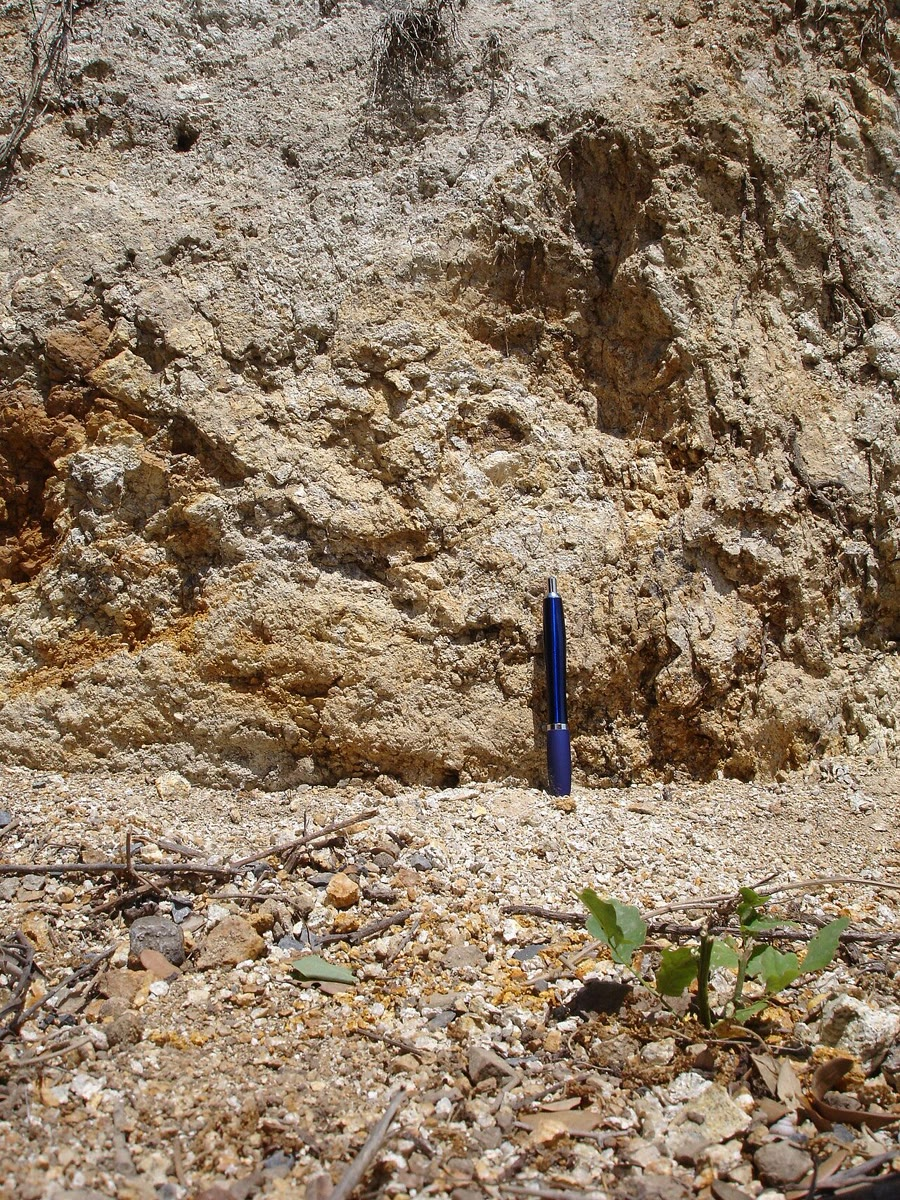
\includegraphics[height=6.3cm]{images/book3/b1-granite-grus.jpg}\hfill
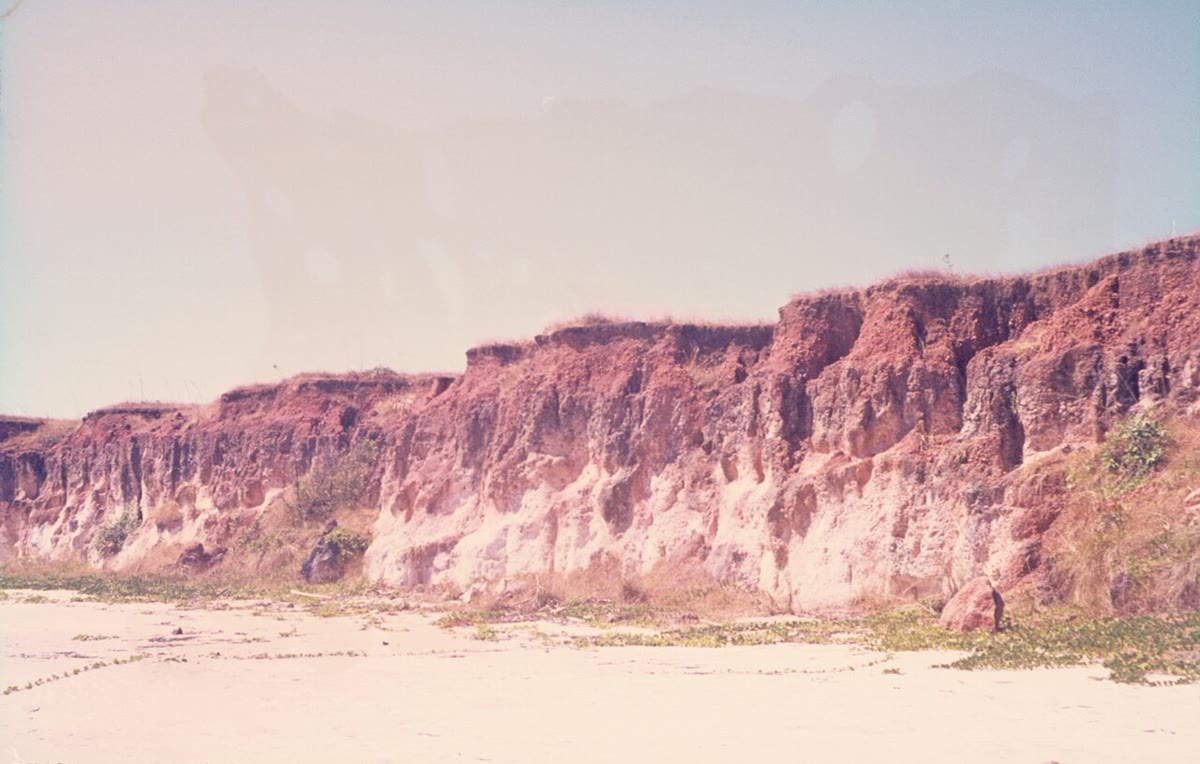
\includegraphics[height=6.3cm]{images/book3/b1-bauxite-weipa.jpg}
{\small يسارًا: جرانيت متفسّخ في جبال البيرينيه، ما زال في مكانه لكنه يتفتّت إلى رمل من الكوارتز \omterm{def:b1:rock-forming-minerals:groups}{والفلسبار} \omterm{def:b1:rock-forming-minerals:groups}{والميكا}، والرمل المفكّك عند قاعدته؛ والقلم يعطي المقياس. تصوير: Pinpin, CC~BY~2.5. ويمينًا: قطاع تجوية على الساحل عند ويبا، شمال أستراليا: بوكسيت أحمر، ناتج \omterm{def:b1:weathering-clays:hydrolysis-degree}{التحلّل الألوميني}، فوق حجر رملي أبيض غني \omterm{def:b1:weathering-clays:clay-mineral}{بالكاولينيت}. تصوير: Werner Schellmann, 1969, CC~BY-SA~2.5. وكلتاهما من ويكيميديا كومنز.}
\label{fig:b1:weathering-clays:photos}
\end{omfigure}
% ledger: commons:grus, commons:weipa

\emph{أيّ \omterm{def:b1:rock-forming-minerals:mineral}{المعادن} تتلاشى أولًا.} في 1938 قارن صموئيل غولديتش القطاعات المتجوّية بصخورها الأصلية، واقترح سلسلة من \omterm{def:b1:rock-forming-minerals:mineral}{المعادن} من الأقلّ إلى الأكثر ثباتًا في التجوية، ووجد أنها تتبع الترتيب الذي تتبلور به من الصهارة: \omterm{def:b1:rock-forming-minerals:groups}{فالأوليفين} \omterm{def:b1:rock-forming-minerals:groups}{والبلاجيوكلاز} الغني بالكالسيوم أولًا، والكوارتز آخرًا. \omterm{def:b1:rock-forming-minerals:mineral}{والمعادن} التي تتكوّن عند أعلى الحرارات أبعد ما تكون عن التوازن على السطح. وقائمة حديثة، من الأقلّ إلى الأكثر مقاومة، هي: البيريت، والكالسيت، والدولوميت، \omterm{def:b1:rock-forming-minerals:groups}{والأوليفين}، \omterm{def:b1:rock-forming-minerals:groups}{والبلاجيوكلاز} الكالسيومي، والبيروكسينات، \omterm{def:b1:rock-forming-minerals:groups}{والبلاجيوكلاز} المتوسط، والأمفيبولات، والبيوتيت، \omterm{def:b1:rock-forming-minerals:groups}{والفلسبار} البوتاسي، والمسكوفيت، \omterm{def:b1:weathering-clays:clay-mineral}{والسميكتيت}، والكوارتز، \omterm{def:b1:weathering-clays:clay-mineral}{والكاولينيت}، والأكسيدان الجيبسيت والهيماتيت. وتؤكّد قياسات المختبر لمعدّلات الذوبان هذا الترتيب؛ ويبقى ترتيبًا، لا قانونًا، لأن معدّل كل \omterm{def:b1:rock-forming-minerals:mineral}{معدن} يتوقّف أيضًا على الماء المحيط به. والنواتج النهائية للتجوية، \omterm{def:b1:weathering-clays:clay-mineral}{الكاولينيت} والجيبسيت والهيماتيت، هي الأكثر مقاومة من الكل: فهي مستقرّة بالفعل على السطح.
% ledger: goldich:1938, formoso:weatherability, lasaga:1984

\emph{ميزان قطاع التجوية.} التجوية تُزيل المادة، لذلك لا يخبرنا تركيز يُقاس في صخر متجوٍّ بمقدار ما فُقد: فخسارة عناصر أخرى تُركّز تلك التي تبقى. والعنصر الذي لا يتحرّك يعطي المرجع.

\begin{proposition}[ميزان الكتلة مع عنصر غير متحرّك]\label{prop:b1:weathering-clays:immobile}
ليكن $i$ عنصرًا لا تحرّكه التجوية، بكسوره الكتلية $C_{i,p}$ في الصخر الأصلي و$C_{i,w}$ في الصخر المتجوّي. فإن كتلة $m_p$ من الصخر الأصلي تصير الكتلة $m_w = m_p C_{i,p}/C_{i,w}$ من الصخر المتجوّي، وكسر ما يُفقد من أي عنصر آخر $j$ هو
\[
  f_j = 1 - \frac{C_{j,w}}{C_{j,p}}\,\frac{C_{i,p}}{C_{i,w}} .
\]
\end{proposition}

\begin{proof}
كتلة $i$ محفوظة: $m_p C_{i,p} = m_w C_{i,w}$، ومنها $m_w$. وكتلة $j$ تنتقل من $m_p C_{j,p}$ إلى $m_w C_{j,w}$، أي يبقى منها كسر
$m_w C_{j,w}/(m_p C_{j,p}) = (C_{j,w}/C_{j,p})(C_{i,p}/C_{i,w})$ ، و$f_j$ هو واحد ناقص هذا الكسر.
\end{proof}

التيتانيوم والزركونيوم هما الاختياران المعتادان، لسبب يعطيه القسم التالي.

\section{أيّ العناصر تغادر: الجهد الأيوني}\label{sec:b1:weathering-clays:ionic}

الصوديوم والبوتاسيوم والكالسيوم تغادر مع الماء؛ والألومنيوم والحديد الثلاثي والتيتانيوم تبقى؛ والسيليكون بينهما. والفرق يكمن في سلوك كل أيون في الماء.

\begin{definition}[الجهد الأيوني]\label{def:b1:weathering-clays:ionic-potential}
\emph{الجهد الأيوني}\index{الجهد الأيوني} للأيون هو النسبة $z/r$ لعدد شحنته $z$ إلى نصف قطره الأيوني $r$، هنا بالأنغستروم (من أجل التنسيق نفسه لكل الأيونات، السداسي فيما يلي).
\end{definition}
% ledger: nomad:goldschmidt, dangic:goldschmidt, shannon:radii-b19

\begin{proposition}[المجالات الثلاثة للجهد الأيوني]\label{prop:b1:weathering-clays:fields}
في ماء التجوية، تبقى الأيونات التي تحقّق $z/r < 3$ في المحلول كأيونات موجبة متميّهة وتُحمل بعيدًا (كاتيونات قابلة للذوبان)؛ والأيونات التي $3 < z/r < 10$ تربط أيونات الهيدروكسيد في الماء، وتترسّب كهيدروكسيدات أو أكاسيد حيث تُطلَق (المتحلّلات المائية)؛ والأيونات التي $z/r > 10$ ترتبط بالأكسجين بقوّة تطرد معها أيونات الهيدروجين، فتنتقل كأكسيأنيونات قابلة للذوبان، مثل الكربونات والكبريتات والفوسفات والنترات. والسيليكون، عند $z/r = 10$، يقع على الحدّ، ويُغسل جزئيًّا، أكثر كلما اشتدّت التجوية.
\end{proposition}
\admitted
% ledger: nomad:goldschmidt, dangic:goldschmidt

القاعدة تجريبية، تعود إلى فيكتور موريتز غولدشميت في الثلاثينيات، وحدودها تقريبية؛ والكيمياء وراءها، أي التجاذب بين كاتيون وأكسجين جزيئات الماء المحيطة به، من اختصاص كتب الكيمياء. فكاتيون صغير مشحون بقوة يجذب إلكترونات جزيئات الماء المحيطة به بشدّة تكفي ليفقد أحدها أيون هيدروجين ويصير هيدروكسيدًا: بقدر معتدل يترسّب الهيدروكسيد؛ وبقدر شديد يفقد الهيدروكسيد نفسه هيدروجينه، فيبقى أكسيأنيون.

يقرأ الرسم أدناه تجوية صخر بنظرة واحدة. فالصوديوم ($z/r = 0.98$)، والبوتاسيوم (0.72)، والكالسيوم (2.0) والمغنيسيوم (2.8) تغادر: فهي الكاتيونات في ماء الأنهار والبحار. ويبقى الألومنيوم (5.6)، والحديد الثلاثي (4.7)، والتيتانيوم (6.6)، والزركونيوم (5.6)، وتتراكم في القطاعات الأشدّ تجوية؛ والتيتانيوم والزركونيوم، اللذان يقعان فوق ذلك في \omterm{def:b1:rock-forming-minerals:mineral}{معادن} تكاد لا تتجوّى، هما المرجعان غير المتحرّكين في \cref{prop:b1:weathering-clays:immobile}. والسيليكون (10.0) هو العنصر الذي تحدّد خسارته الجزئية درجات \omterm{def:b1:weathering-clays:hydrolysis}{التحلّل المائي}.
% ledger: shannon:radii-b19

والأكسدة تنقل أيونًا عبر الحدّ. فالحديد الثنائي، عند $z/r = 2.6$، كاتيون قابل للذوبان؛ والحديد الثلاثي، عند 4.7، متحلّل مائي. ففي تربة مشبّعة بالماء بلا أكسجين، يذوب الحديد ك\ce{Fe^2+} ويُحمل بعيدًا، فتبقى التربة رمادية؛ وحيث يلتقي الماء بالهواء، عند نبع أو في تربة جيدة التصريف، يتأكسد الحديد ويترسّب فورًا كأكاسيد حمراء وبنّية. والمنغنيز يسلك السلوك نفسه، \ce{Mn^2+} (2.4) مقابل \ce{Mn^4+} (7.5).
% ledger: nomad:goldschmidt, shannon:radii-b19

\begin{omfigure}
\begin{tikzpicture}[font=\small]
% ionic-potential diagram (figdata/bachelor-1/ionic_potential.py): charge against Shannon radius
\begin{axis}[width=12.5cm, height=8.4cm, xmin=0, xmax=1.8, ymin=0, ymax=7,
    xlabel={نصف القطر الأيوني $r$ (\si{\angstrom}، تنسيق سداسي)}, ylabel={الشحنة $z$},
    ytick={1,...,6}, xtick={0,0.2,...,1.8}, xticklabel style={/pgf/number format/fixed},
    axis on top, clip=true]
  \fill[omThm!14] (axis cs:0,0) -- (axis cs:1.8,0) -- (axis cs:1.8,5.4) -- cycle;
  \fill[omDef!16] (axis cs:0,0) -- (axis cs:1.8,5.4) -- (axis cs:1.8,7) -- (axis cs:0.7,7) -- cycle;
  \fill[omExo!18] (axis cs:0,0) -- (axis cs:0.7,7) -- (axis cs:0,7) -- cycle;
  \addplot[black, thick] table[x=r, y=z3] {figdata/out/bachelor-1-ionic_potential-lines.dat};
  \addplot[black, thick] table[x=r, y=z10] {figdata/out/bachelor-1-ionic_potential-lines.dat};
  \addplot[only marks, mark=*, mark size=1.6pt, black,
      point meta=explicit symbolic, nodes near coords,
      visualization depends on={value \thisrow{anc} \as \anc},
      every node near coord/.append style={font=\scriptsize, inner sep=2.6pt, anchor=\anc}]
    table[x=r, y=z, meta=tex] {figdata/out/bachelor-1-ionic_potential-ions.dat};
  \node[font=\footnotesize, align=center, fill=white, fill opacity=0.8, text opacity=1, rounded corners=1pt] at (axis cs:1.45,2.75) {كاتيونات قابلة للذوبان\\ $z/r < 3$};
  \node[font=\footnotesize, align=center, fill=white, fill opacity=0.8, text opacity=1, rounded corners=1pt] at (axis cs:1.15,6.3) {متحلّلات مائية\\ $3 < z/r < 10$};
  \node[font=\footnotesize, align=left, fill=white, fill opacity=0.8, text opacity=1, rounded corners=1pt, anchor=north west] at (axis cs:0.015,6.95) {أكسيأنيونات قابلة للذوبان، $z/r > 10$};
  \node[font=\scriptsize, rotate=28, anchor=south] at (axis cs:1.62,4.86) {$z/r = 3$};
  \node[font=\scriptsize, rotate=61, anchor=south] at (axis cs:0.2,2.0) {$z/r = 10$};
\end{axis}
\end{tikzpicture}

{\small مخطط \omterm{def:b1:weathering-clays:ionic-potential}{الجهد الأيوني}: كل أيون موضوع حسب نصف قطره الأيوني الفعّال في تنسيق سداسي (شانون، 1976) وشحنته. والخطّان $z/r = 3$ و$z/r = 10$ يفصلان الأيونات التي تغادر في المحلول ككاتيونات، وتلك التي تبقى كهيدروكسيدات أو أكاسيد، وتلك التي تغادر كأكسيأنيونات. والسيليكون يقع على الحدّ الأعلى.}
\label{fig:b1:weathering-clays:ionic-potential}
\end{omfigure}
% ledger: shannon:radii-b19, nomad:goldschmidt

\section{المعادن الطينية}\label{sec:b1:weathering-clays:clays}

\begin{definition}[المعدن الطيني، والكاولينيت، والإيليت، والسميكتيت، والكلوريت]\label{def:b1:weathering-clays:clay-mineral}
\emph{المعدن الطيني}\index{المعدن الطيني} هو سيليكات صفائحية ألومنيومية مائية، عادةً في حبيبات بعرض بضعة ميكرومترات أو أقلّ، مبنية من طبقات تجمع صفيحة رباعية (T) من رباعيات الأوجه \ce{SiO4} تتشارك ثلاثة أركان، وصفيحة ثمانية (O) من الألومنيوم أو المغنيسيوم محاطة بالأكسجين والهيدروكسيل. ففي \emph{الكاولينيت}\index{الكاولينيت}، \ce{Al2Si2O5(OH)4}، كل طبقة صفيحة T وصفيحة O واحدة (طبقة 1:1 أو T--O)، متعادلة، والطبقات تتماسك بروابط هيدروجينية. وفي \omterm{def:b1:rock-forming-minerals:mineral}{المعادن} الطينية 2:1 أو T--O--T تقع صفيحة O بين صفيحتي T تشيران نحوها: ف\emph{الإيليت}\index{الإيليت} \omterm{def:b1:rock-forming-minerals:mineral}{معدن} طيني 2:1 غير متمدّد، فيه أيونات بوتاسيوم بين الطبقات، \omterm{def:b1:rock-forming-minerals:groups}{كالميكا} بقدر أقلّ من البوتاسيوم؛ و\emph{السميكتيت}\index{السميكتيت} \omterm{def:b1:rock-forming-minerals:mineral}{معدن} طيني 2:1 فيه كاتيونات متميّهة قابلة للتبادل، وماء بين طبقاته، يستطيع أن يمتصّ مزيدًا من الماء فينتفخ؛ و\emph{الكلوريت}\index{الكلوريت} \omterm{def:b1:rock-forming-minerals:mineral}{معدن} 2:1 تتناوب طبقاته السالبة الشحنة مع صفائح ثمانية موجبة الشحنة من نوع البروسيت، \ce{(Mg,Fe)(OH)2} مع بعض الألومنيوم.
\end{definition}
% ledger: usgs:clay-groups, usgs:clay-settings, webmineral:clays-b19, biscaye:1965

طبقة الشحنة تحدّد كيف تتكدّس الطبقات، والشحنة تأتي من الاستبدالات في الصفائح (\cref{def:b1:rock-forming-minerals:substitution}).

\begin{proposition}[شحنة طبقة 2:1]\label{prop:b1:weathering-clays:layer-charge}
طبقة 2:1 صيغتها $\mathrm{(Si_{4-x}Al_x)(Al_{2-y}Mg_y)O_{10}(OH)_2}$، حيث $x$ ألومنيوم محلّ السيليكون في صفائحها الرباعية و$y$ مغنيسيوم محلّ الألومنيوم في صفيحتها الثمانية، تحمل الشحنة $-(x + y)$ لكل وحدة صيغية.
\end{proposition}

\begin{proof}
اجمع الشحنات: $4(4 - x) + 3x$ من الكاتيونات الرباعية، و$3(2 - y) + 2y$ من الثمانية، و$-2\times10$ من الأكسجين و$-1\times2$ من الهيدروكسيلات: $16 - x + 6 - y - 20 - 2 = -(x + y)$.
\end{proof}

من دون استبدال ($x = y = 0$) تكون الطبقة متعادلة، كما في \ce{Al2Si4O10(OH)2}، \omterm{def:b1:rock-forming-minerals:mineral}{معدن} البيروفيلايت، وتتماسك الطبقات بقوى ضعيفة فقط. وفي المسكوفيت، $x = 1$، فالشحنة $-1$ يوازنها أيون بوتاسيوم واحد يُحكم قفل الطبقات معًا؛ \omterm{def:b1:weathering-clays:clay-mineral}{والإيليت} قريب منه، بقليل أقلّ. وفي البيدلايت من \cref{prop:b1:weathering-clays:feldspars}، $x = 0.5$: فالشحنة $-0.5$ يوازنها $0.5$ من الصوديوم. والشحنة الأصغر تُمسك الطبقات بإحكام أقلّ، ويمكن أن يدخل بينها ماء وكاتيونات متميّهة: ولهذا تنتفخ السميكتيتات، بشحنات نحو 0.3 إلى 0.5 لكل وحدة صيغية، كما في صيغتي المونتموريلونيت والبيدلايت، ولا ينتفخ \omterm{def:b1:weathering-clays:clay-mineral}{الإيليت}. والكاتيونات بين طبقات \omterm{def:b1:weathering-clays:clay-mineral}{السميكتيت} قابلة للتبادل، وسعة التبادل \omterm{def:b1:rock-forming-minerals:mineral}{للمعادن} الطينية الشائعة تتبع بنيتها: من 3 إلى 15 مللي مكافئ لكل \qty{100}{g} \omterm{def:b1:weathering-clays:clay-mineral}{للكاولينيت}، الذي لا تحمل طبقاته شحنة، ومن 10 إلى 40 \omterm{def:b1:weathering-clays:clay-mineral}{للإيليت}، ومن 70 إلى 100 للمونتموريلونيت، وهو \omterm{def:b1:weathering-clays:clay-mineral}{سميكتيت}. والبوتاسيوم، الذي يُحكم قفل طبقات \omterm{def:b1:rock-forming-minerals:groups}{الميكا}، يفضّل \omterm{def:b1:weathering-clays:clay-mineral}{الإيليت}؛ وتتكوّن السميكتيتات حيث يكون البوتاسيوم شحيحًا ويتوفّر الكالسيوم والمغنيسيوم.
% ledger: webmineral:clays-b19, carroll:cec, usgs:clay-settings

\begin{omfigure}
\begin{tikzpicture}[font=\footnotesize, >={Stealth[length=4pt]}, y=0.2cm, x=1cm]
% schematic clay-mineral structures, vertical scale proportional to the basal spacings
% (USGS OFR 01-041, ledger usgs:clay-xrd): kaolinite 7, illite 10, smectite 14 (air-dried), chlorite 14 angstrom.
% T sheet 2 A thick, O sheet 2.4 A thick (schematic); the column width is 2.2 cm.
\def\W{2.2}
\newcommand{\Tsheet}[1]{% tetrahedral sheet whose base is at y=#1
  \fill[omDef!35] (0,#1) rectangle (\W,#1+2);
  \foreach \i in {0,...,6} {\draw[omDef!80!black, line width=0.4pt] (0.04+\i*0.31,#1) -- (0.195+\i*0.31,#1+2) -- (0.35+\i*0.31,#1) -- cycle;}
}
\newcommand{\TsheetDown}[1]{% inverted tetrahedral sheet, base at the top (y=#1+2)
  \fill[omDef!35] (0,#1) rectangle (\W,#1+2);
  \foreach \i in {0,...,6} {\draw[omDef!80!black, line width=0.4pt] (0.04+\i*0.31,#1+2) -- (0.195+\i*0.31,#1) -- (0.35+\i*0.31,#1+2) -- cycle;}
}
\newcommand{\Osheet}[2]{% octahedral sheet, base at y=#1, fill colour #2
  \fill[#2] (0,#1) rectangle (\W,#1+2.4);
  \foreach \i in {0,...,4} {\draw[black!55, line width=0.4pt] (0.17+\i*0.42,#1+1.2) -- ++(0.17,1.0) -- ++(0.17,-1.0) -- ++(-0.17,-1.0) -- cycle;}
}
\newcommand{\spacing}[3]{% arrow for d001 from y=#1 to y=#2 with label #3
  \draw[<->, line width=0.5pt] (\W+0.18,#1) -- (\W+0.18,#2) node[midway, right, inner sep=2pt] {#3};
  \draw[black!40, densely dotted] (\W,#1) -- (\W+0.28,#1); \draw[black!40, densely dotted] (\W,#2) -- (\W+0.28,#2);
}
% ---------- kaolinite: T-O, d = 7.2
\begin{scope}[xshift=0cm]
  \foreach \b in {0, 7.2} {\Tsheet{\b} \Osheet{\b+2}{omThm!25}}
  \spacing{0}{7.2}{\SI{7}{\angstrom}}
  \node[anchor=north, align=center] at (\W/2,-0.8) {\textbf{الكاولينيت}\\ طبقات T--O (1:1)\\ تتماسك بروابط هيدروجينية};
\end{scope}
% ---------- illite: T-O-T + K, d = 10
\begin{scope}[xshift=3.6cm]
  \foreach \b in {0, 10} {\Tsheet{\b} \Osheet{\b+2}{omThm!25} \TsheetDown{\b+4.4}}
  \foreach \b in {6.4} {\foreach \i in {0,...,4} \fill[omExo!70!black] (0.25+\i*0.42,\b+1.8) circle[radius=1.5pt];}
  \spacing{0}{10}{\SI{10}{\angstrom}}
  \node[anchor=north, align=center] at (\W/2,-0.8) {\textbf{الإيليت}\\ طبقات T--O--T (2:1)\\ تتماسك بأيونات \ce{K+}};
\end{scope}
% ---------- smectite: T-O-T + hydrated cations, d = 14
\begin{scope}[xshift=7.2cm]
  \foreach \b in {0, 14} {\Tsheet{\b} \Osheet{\b+2}{omThm!25} \TsheetDown{\b+4.4}}
  \foreach \i in {0,...,9} {\draw[omDef!60, line width=0.3pt] (0.13+\i*0.215,8.6) circle[radius=1.3pt]; \draw[omDef!60, line width=0.3pt] (0.2+\i*0.215,11.8) circle[radius=1.3pt];}
  \foreach \i in {0,...,3} {\fill[omExo!70!black] (0.35+\i*0.5,10.2) circle[radius=1.5pt];}
  \spacing{0}{14}{\SI{14}{\angstrom}}
  \node[anchor=north, align=center] at (\W/2,-0.8) {\textbf{السميكتيت}\\ طبقات T--O--T، متميّهة\\ \ce{Na+}، \ce{Ca^2+} وماء};
\end{scope}
% ---------- chlorite: T-O-T + brucite-like O sheet, d = 14
\begin{scope}[xshift=10.8cm]
  \foreach \b in {0, 14} {\Tsheet{\b} \Osheet{\b+2}{omThm!25} \TsheetDown{\b+4.4}}
  \Osheet{9}{omExo!25}
  \spacing{0}{14}{\SI{14}{\angstrom}}
  \node[anchor=north, align=center] at (\W/2,-0.8) {\textbf{الكلوريت}\\ طبقات T--O--T وصفيحة O\\ من نوع البروسيت};
\end{scope}
% key
\begin{scope}[xshift=0cm, yshift=-2.75cm]
  \fill[omDef!35] (0,0) rectangle (0.4,1.6); \draw[omDef!80!black] (0.05,0) -- (0.2,1.6) -- (0.35,0) -- cycle;
  \node[anchor=west] at (0.5,0.8) {T: صفيحة رباعية، \ce{SiO4} (وبعض \ce{AlO4})};
  \fill[omExo!70!black] (8.1,0.8) circle[radius=1.5pt]; \node[anchor=west] at (8.3,0.8) {كاتيون بين الطبقات};
  \fill[omThm!25] (0,-2.6) rectangle (0.4,-1.0);
  \node[anchor=west] at (0.5,-1.8) {O: صفيحة ثمانية، \ce{Al} أو \ce{Mg} مع \ce{O} و\ce{OH}};
  \draw[omDef!60] (8.1,-1.8) circle[radius=1.3pt]; \node[anchor=west] at (8.3,-1.8) {جزيء ماء};
\end{scope}
\end{tikzpicture}

{\small أنواع \omterm{def:b1:rock-forming-minerals:mineral}{المعادن} الطينية الأربعة (تخطيطية، طبقتان من كل نوع). المقياس الشاقولي يتناسب مع المسافة القاعدية، أي المسافة الدورية من طبقة إلى التالية، كما تقيسها حيود الأشعة السينية: \SI{7}{\angstrom} \omterm{def:b1:weathering-clays:clay-mineral}{للكاولينيت}، و\SI{10}{\angstrom} \omterm{def:b1:weathering-clays:clay-mineral}{للإيليت}، ونحو \SI{14}{\angstrom} \omterm{def:b1:weathering-clays:clay-mineral}{لسميكتيت} مجفّف بالهواء ولكلوريت.}
\label{fig:b1:weathering-clays:structures}
\end{omfigure}
% ledger: usgs:clay-xrd, usgs:clay-groups



\begin{table}[htbp]
\centering\footnotesize
\setlength{\tabcolsep}{4pt}
% ledger: usgs:clay-xrd, usgs:clay-groups, usgs:clay-settings, carroll:cec, biscaye:1965
\begin{tabular}{@{}>{\raggedright\arraybackslash}p{1.6cm}>{\raggedright\arraybackslash}p{1.5cm}>{\raggedright\arraybackslash}p{1.6cm}>{\raggedright\arraybackslash}p{1.5cm}>{\raggedright\arraybackslash}p{1.4cm}>{\raggedright\arraybackslash}p{1.4cm}>{\raggedright\arraybackslash}p{1.2cm}>{\raggedright\arraybackslash}p{3.2cm}@{}}
\hline
\omterm{def:b1:rock-forming-minerals:mineral}{المعدن} & الطبقة & ما بين الطبقات & مجفّف بالهواء & الغليكول & التسخين & سعة التبادل & الوسط المعتاد \\
\hline
\omterm{def:b1:weathering-clays:clay-mineral}{الكاولينيت} & T--O & لا شيء & \SI{7}{\angstrom} & \SI{7}{\angstrom} & يتلف عند \SI{550}{\celsius} & 3--15 & فلسبارات يغسلها ماء حمضي؛ تجوية استوائية شديدة \\
\omterm{def:b1:weathering-clays:clay-mineral}{الإيليت} & T--O--T & \ce{K+} & \SI{10}{\angstrom} & \SI{10}{\angstrom} & \SI{10}{\angstrom} & 10--40 & ماء قلوي غني بالبوتاسيوم؛ من الفلسبارات والميكات؛ الطين الرئيسي للطفل \\
\omterm{def:b1:weathering-clays:clay-mineral}{السميكتيت} & T--O--T & \ce{Na+}، \ce{Ca^2+} متميّهة & نحو \SI{14}{\angstrom} & \SI{17}{\angstrom} & \SI{10}{\angstrom} عند \SI{400}{\celsius} & 70--100 & صخور قاعدية متجوّية؛ أرض رديئة التصريف، والبوتاسيوم شحيح \\
\omterm{def:b1:weathering-clays:clay-mineral}{الكلوريت} & T--O--T & صفيحة من نوع البروسيت & \SI{14}{\angstrom} & \SI{14}{\angstrom} & \SI{14}{\angstrom} & -- & صخور متحوّلة منخفضة الدرجة وصخور نارية متغيّرة؛ طفل \\
\hline
\end{tabular}
\caption{أسر \omterm{def:b1:rock-forming-minerals:mineral}{المعادن} الطينية الأربع: البنية، والمسافة القاعدية المقاسة على عيّنات موجّهة مجفّفة بالهواء، وبعد التشبّع بالغليكول الإيثيلي وبعد التسخين، وسعة التبادل الكاتيوني (مللي مكافئ لكل \qty{100}{g}؛ والقيمة \omterm{def:b1:weathering-clays:clay-mineral}{للسميكتيت} هي قيمة المونتموريلونيت)، والأماكن التي تتكوّن فيها عادةً.}
\label{tab:b1:weathering-clays:clays}
\end{table}

\begin{inthelab}[تعريف المعادن الطينية بحيود الأشعة السينية]
\omterm{def:b1:rock-forming-minerals:mineral}{المعادن} الطينية أدقّ من أن تُفرَّق تحت المجهر الضوئي. وفي المختبر يُفصل أدقّ جزء من تربة أو من طفل بترك الحبيبات الأخشن تترسّب من الماء، وتُجفَّف قطرة من المعلّق على شريحة زجاجية حيث تستلقي الرقائق مسطّحة: وهذه عيّنة موجّهة. والأشعة السينية المنعكسة من الطبقات المتراصّة تعطي قممًا قوية عند الزوايا التي يحدّدها البُعد القاعدي، بقانون براغ للحيود (الفيزياء). وتُشغَّل الشريحة ثلاث أو أربع مرات: مجفّفة بالهواء؛ وبعد ليلة في بخار الغليكول الإيثيلي، الذي يدخل ما بين طبقات السميكتيتات ويُنفخها إلى \SI{17}{\angstrom} تاركًا \omterm{def:b1:rock-forming-minerals:mineral}{المعادن} الأخرى دون تغيير؛ وبعد التسخين إلى \SI{400}{\celsius}، الذي يُخرج الماء من السميكتيتات ويضغطها إلى \SI{10}{\angstrom}؛ وبعد التسخين إلى \SI{550}{\celsius}، الذي يدمّر \omterm{def:b1:weathering-clays:clay-mineral}{الكاولينيت} لكنه يترك \omterm{def:b1:weathering-clays:clay-mineral}{الإيليت} \omterm{def:b1:weathering-clays:clay-mineral}{والكلوريت}. و\Cref{tab:b1:weathering-clays:clays} هو مفتاح قراءة التشغيلات الأربعة؛ أما الخلائط \omterm{def:b1:rock-forming-minerals:mineral}{والمعادن} المتداخلة الطبقات، وهي شائعة جدًّا في التربات، فتحتاج إلى أكثر من ذلك.
\end{inthelab}
% ledger: usgs:clay-xrd

\begin{omfigure}
\begin{minipage}[t]{0.66\linewidth}\vspace{0pt}
\emph{الطين مؤشرًا مناخيًّا.} لأن درجة \omterm{def:b1:weathering-clays:hydrolysis}{التحلّل المائي} تتبع المناخ، فإن \omterm{def:b1:rock-forming-minerals:mineral}{المعادن} الطينية في التربة تسجّله: \omterm{def:b1:weathering-clays:clay-mineral}{فالكاولينيت} والجيبسيت حيث تكون التجوية شديدة، تحت مناخات حارّة رطبة؛ والسميكتيتات حيث يتجدّد الماء قليلًا؛ وحيث تكون التجوية ضعيفة، تكون الطين موروثًا في معظمه من الصخر، \omterm{def:b1:weathering-clays:clay-mineral}{فالإيليت} \omterm{def:b1:weathering-clays:clay-mineral}{والكلوريت} من الميكات والشست. وتحمل الأنهار هذه الطين إلى البحر، وتحفظ طينُ قاع البحر السجلّ: فقبالة الأنهار الصغيرة في أمريكا الجنوبية الاستوائية، الغنية \omterm{def:b1:weathering-clays:clay-mineral}{بالكاولينيت} والجيبسيت، يُرى التجوية الشديدة للأرض التي تصرّفها. وحين تُدفن التربات وتُحفظ، تُستعمل معادنها الطينية لاستنتاج مناخات الماضي الجيولوجي: فطبقة غنية \omterm{def:b1:weathering-clays:clay-mineral}{بالكاولينيت} في سلسلة من الطفل الغني \omterm{def:b1:weathering-clays:clay-mineral}{بالإيليت} تشير إلى حقبة دافئة رطبة. ويحتاج هذا الاستنتاج إلى عناية، لأن \omterm{def:b1:rock-forming-minerals:mineral}{المعادن} الطينية تُنقل أيضًا بعيدًا عن مكان تكوّنها، ويحوّلها الدفن: فالسميكتيتات تصير إيليتًا حين تسخن (\cref{ch:b1:diagenesis-basins}).
\end{minipage}\hfill
\begin{minipage}[t]{0.30\linewidth}\vspace{0pt}
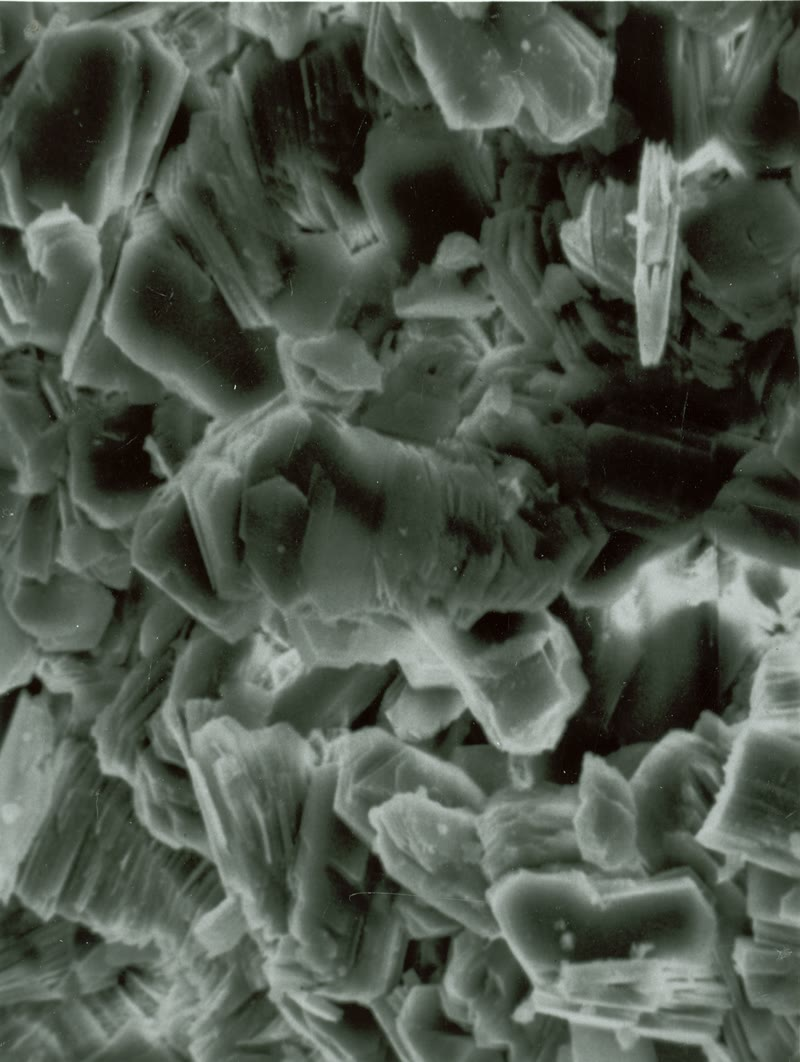
\includegraphics[width=\linewidth]{images/book3/b1-kaolinite-sem.jpg}

{\scriptsize \omterm{def:b1:weathering-clays:clay-mineral}{كاولينيت} كما يُرى بالمجهر الإلكتروني الماسح: كتب من صفائح سداسية متراكمة نمت في مسامّ حجر رملي من شمال ألاسكا (تكبير نحو 1340). هيئة المسح الجيولوجي الأمريكية، U.S. Geological Survey, ملك عام، عبر ويكيميديا كومنز.\par}
\end{minipage}
\end{omfigure}
% ledger: biscaye:1965, usgs:clay-settings, pedron:stages, commons:kaolinite-sem

\emph{اللاتيريتات.} حيث يبلغ \omterm{def:b1:weathering-clays:hydrolysis}{التحلّل المائي} درجاته الأخيرة زمنًا طويلًا، يسمك القطاع وتتركّز في أعلاه كل المادة التي لا تغادر.

\begin{definition}[اللاتيريت]\label{def:b1:weathering-clays:laterite}
\emph{اللاتيريت}\index{اللاتيريت} هو الناتج الغني بالحديد والألومنيوم للتحلّل المائي الشديد والطويل تحت مناخات حارّة رطبة: مادة حمراء إلى بنّية، لينة أو متصلّبة، مؤلّفة من \omterm{def:b1:weathering-clays:clay-mineral}{الكاولينيت} وأكاسيد الحديد وهيدروكسيداته، مع الجيبسيت حيث يُبلغ \omterm{def:b1:weathering-clays:hydrolysis-degree}{التحلّل الألوميني}، وقد أُزيلت منها كل الكاتيونات القلوية والقلوية الترابية تقريبًا، وكثير من السيليكا.
\end{definition}
% ledger: formoso:laterite, buchanan:laterite

\omterm{def:b1:weathering-clays:laterite}{واللاتيريت} الغني بالجيبسيت أو البوهميت، هيدروكسيدَي الألومنيوم، هو بوكسيت، خام تسعة أعشار الألومنيوم: \omterm{def:b1:weathering-clays:hydrolysis-degree}{والتحلّل الألوميني} هو الخطوة التي تصنع الخام. وأكثر البوكسيتات متبقّية، أي الصخر الذي أُزيل منه كل شيء عدا الألومينا؛ ومعظم ما هو مؤلّف من الجيبسيت يقع في المناطق الاستوائية، وكثير منها على الأرجح ما زال يتكوّن.
% ledger: usgs:bauxite

\begin{history}[كلمة من الميدان]
في 1807 وصف فرانسيس بوكانان، وهو يسافر في مالابار، جنوب الهند، مادةً مليئةً بالتجاويف وغنيةً بمغرات الحديد الحمراء والصفراء، منتشرةً فوق الجرانيت في كتل كبيرة. وحين أُخرجت من الأرض كانت لينة إلى حدّ أن سكّينًا تقطعها، فكان السكان يشكّلونها كتلًا؛ وفي الهواء تصير سريعًا صلبة كالطوب، وتدوم أفضل من أيّ طوب رآه. وكانت اللغات المحلية تسمّيها حجر الطوب؛ فاقترح اسم \omterm{def:b1:weathering-clays:laterite}{اللاتيريت}، الذي حفظته الجيولوجيا للنواتج الحمراء للتجوية الاستوائية.
\end{history}
% ledger: buchanan:laterite

\section{التجوية السيليكاتية وثاني أكسيد الكربون}\label{sec:b1:weathering-clays:co2}

أيونات الهيدروجين في \omterm{def:b1:weathering-clays:hydrolysis}{التحلّل المائي} تأتي في معظمها من ثاني أكسيد الكربون، لذلك فكتابتها كحمض الكربونيك تبيّن ما تفعله التجوية بالهواء. ولسيليكات كالسيوم، تُكتب \ce{CaSiO3} للتبسيط،
\[
  \ce{CaSiO3 + 2 CO2 + H2O -> Ca^2+ + 2 HCO3- + SiO2},
\]
وفي المحيط، حيث تبني الكائنات أصدافًا من كربونات الكالسيوم،
\[
  \ce{Ca^2+ + 2 HCO3- -> CaCO3 + CO2 + H2O}.
\]

\begin{proposition}[التجوية وثاني أكسيد الكربون]\label{prop:b1:weathering-clays:co2}
(أ) تجوية سيليكات تستهلك مولين من ثاني أكسيد الكربون، يتحوّل إلى بيكربونات، لكل مول من الكالسيوم أو المغنيسيوم المحرَّر؛ وحين يترسّب الكالسيوم أو المغنيسيوم ككربونات، يعود أحد المولين إلى الهواء، ويُخزَّن مول واحد كصخر كربوناتي. (ب) تجوية صخر كربوناتي وترسيب كربوناته من جديد لا يخزّن شيئًا.
\end{proposition}

\begin{proof}
(أ) بجمع المعادلتين أعلاه يعطي \ce{CaSiO3 + CO2 -> CaCO3 + SiO2}: يغادر الهواء \ce{CO2} واحد لكل كالسيوم نهائيًا؛ والمعادلة الأولى وحدها تبيّن أن اثنين استُهلكا. والأمر نفسه للمغنيسيوم، مع \ce{Mg^2+} بدل \ce{Ca^2+}. (ب) ذوبان الكالسيت، \ce{CaCO3 + CO2 + H2O -> Ca^2+ + 2
HCO3-}، هو عكس الترسيب تمامًا: فمجموع المعادلتين صفر.
\end{proof}

مع \omterm{def:b1:rock-forming-minerals:groups}{الفلسبار}، يحلّ حمض الكربونيك محلّ أيونات الهيدروجين في \cref{prop:b1:weathering-clays:feldspars}: فكل \ce{H+} مُستهلَك هو \ce{CO2} واحد تحوّل إلى \ce{HCO3-}. فالأنورثيت من البازلت أو الغابرو يستهلك إذن مولين من ثاني أكسيد الكربون لكل مول بينما يتحوّل إلى \omterm{def:b1:weathering-clays:clay-mineral}{الكاولينيت}،
\[
  \ce{CaAl2Si2O8 + 2 CO2 + 3 H2O -> Al2Si2O5(OH)4 + Ca^2+ + 2 HCO3-},
\]
ويُخزَّن واحد منه على المدى الطويل. ولا يكوّن الصوديوم والبوتاسيوم كربونات في قاع البحر، ويُحسب التخزين طويل المدى من الكالسيوم والمغنيسيوم المحرَّرين.

وتحمل الأنهار البيكربونات إلى البحر، وكيمياؤها تقيس التدفّق. ومن كيمياء أنهار العالم الكبيرة، قُدّر ثاني أكسيد الكربون المستهلك بتجوية السيليكات القارية بين \num{11.7e12} و\qty{13.6e12}{mol} في السنة، أي نحو 0.14 إلى 0.16 مليار طن من الكربون، منها تجوية البازلت وحدها تفسّر من 30 إلى \qty{35}{\percent}. والتدفّق صغير أمام التبادلات الكربونية بين الهواء والمحيطات والكائنات الحية، لكنه لا ينعكس: فعلى مدى ملايين السنين هو الطريقة الرئيسية التي يغادر بها الهواء ثاني أكسيد الكربون الذي تضخّه البراكين. ولأن التجوية تجري أسرع حين تكون أدفأ وأرطب، فهي تربط ثاني أكسيد الكربون في الهواء بالمناخ، الذي يتوقّف بدوره على ثاني أكسيد الكربون عبر تأثير الاحتباس الحراري: تغذية راجعة سالبة تُثبّت حرارة الأرض عبر الزمن الجيولوجي، ويدرسها مجلد السنة الثانية.
% ledger: dessert:silicate-co2, whk:1981

\section{التمارين}

\begin{exercise}[$\star$]\label{exo:b1:weathering-clays:1}
باستعمال نصف الأقطار \ce{K+} \qty{1.38}{\angstrom}، و\ce{Fe^2+} \qty{0.78}{\angstrom}،
\ce{Fe^3+} \qty{0.645}{\angstrom} و\ce{Ti^4+} \qty{0.605}{\angstrom}، احسب \omterm{def:b1:weathering-clays:ionic-potential}{الجهد الأيوني} لكل أيون وسمِّ مجاله. لماذا تفقد تربة مشبعة بالماء حديدها، بينما تحتفظ به تربة جيدة التصريف؟
% ledger: shannon:radii-b19
\end{exercise}

\begin{exercise}[$\star$]\label{exo:b1:weathering-clays:2}
أربعة أجزاء طينية تُعرَّض للأشعة السينية كعيّنات موجّهة. A: قمة عند
\SI{14}{\angstrom}، تنتقل إلى \SI{17}{\angstrom} بالغليكول، وإلى
\SI{10}{\angstrom} بالتسخين إلى \SI{400}{\celsius}. B: قمة عند
\SI{7}{\angstrom}، لا يغيّرها الغليكول، وتختفي بعد التسخين إلى
\SI{550}{\celsius}. C: قمة عند \SI{10}{\angstrom} لا تحرّكها أيّ معاملة. D:
قمة عند \SI{14}{\angstrom} لا تحرّكها أيّ معاملة. عرّف كل \omterm{def:b1:rock-forming-minerals:mineral}{معدن}.
% ledger: usgs:clay-xrd
\end{exercise}

\begin{exercise}[$\star$]\label{exo:b1:weathering-clays:3}
بموازنة ذلك ب\cref{met:b1:weathering-clays:balance}، حلّل \omterm{def:b1:weathering-clays:hydrolysis}{التحلّل المائي} للأورثوكلاز \ce{KAlSi3O8} إلى \omterm{def:b1:weathering-clays:clay-mineral}{الكاولينيت}. ما كسر بوتاسيومه وسيليكونه الذي يغادر في المحلول؟
\end{exercise}

\begin{exercise}[$\star$]\label{exo:b1:weathering-clays:4}
(أ) ما حجم الجليد الذي يعطيه \qty{10}{cm^3} من الماء عند \qty{0}{\celsius}؟ (ب) ضمن أيّ مدى من الحرارة يفلق الجليد النامي في الشقوق الصخرَ أكثر فاعلية، ولماذا لا يفعل ذلك صقيع أخفّ أو أقسى؟ (ج) مكعب من الجرانيت طول ضلعه \qty{1}{m} يفلقه الصقيع إلى مكعبات طول ضلعها \qty{1}{cm}: بأيّ عامل نما سطحه؟
% ledger: usgs:water-density, iapws:ice-density, wh85:frost
\end{exercise}

\begin{exercise}[$\star\star$]\label{exo:b1:weathering-clays:5}
احسب السطح النوعي لحبيبات \omterm{def:b1:rock-forming-minerals:groups}{الفلسبار} كثافتها \qty{2600}{kg.m^{-3}}، معاملةً كمكعبات، لأحجام \qty{1}{cm}، و\qty{1}{mm}، و\qty{1}{\micro m}. لماذا يهمّ حجم الحبيبة كثيرًا لمعدّل \omterm{def:b1:weathering-clays:weathering}{التجوية الكيميائية}، ولماذا تسرّع \omterm{def:b1:weathering-clays:weathering}{التجوية الفيزيائية} \omterm{def:b1:weathering-clays:weathering}{التجوية الكيميائية}؟
\end{exercise}

\begin{exercise}[$\star\star$]\label{exo:b1:weathering-clays:6}
طنّ من \ce{NaAlSi3O8} (\qty{262.22}{g.mol^{-1}}) من الألبيت يتحوّل إلى \omterm{def:b1:weathering-clays:clay-mineral}{الكاولينيت} (\qty{258.16}{g.mol^{-1}}). احسب كتلة \omterm{def:b1:weathering-clays:clay-mineral}{الكاولينيت} المتكوّن، وكتلة السيليكا المُصدَّرة، محسوبةً ك\ce{SiO2} (\qty{60.08}{g.mol^{-1}})، وكتلة الصوديوم المُصدَّر.
% ledger: webmineral:clays-b19, ciaaw:Na
\end{exercise}

\begin{exercise}[$\star\star$]\label{exo:b1:weathering-clays:7}
يحتوي جرانيت، بالكتلة، على \qty{0.30}{\percent} \ce{TiO2}، و\qty{3.5}{\percent} \ce{Na2O}، و\qty{72}{\percent} \ce{SiO2}، و\qty{14}{\percent} \ce{Al2O3}؛ وسابرولايته يحتوي \qty{0.60}{\percent} \ce{TiO2}، و\qty{0.35}{\percent} \ce{Na2O}، و\qty{60}{\percent} \ce{SiO2}، و\qty{27}{\percent} \ce{Al2O3}. مع اعتبار التيتانيوم غير متحرّك، احسب كتلة السابرولايت الباقية من كيلوغرام من الجرانيت، وكسر الصوديوم والسيليكون والألومنيوم المفقود. وأيّ درجة من \omterm{def:b1:weathering-clays:hydrolysis}{التحلّل المائي} جارية؟
\end{exercise}

\begin{exercise}[$\star\star$]\label{exo:b1:weathering-clays:8}
باستعمال \cref{prop:b1:weathering-clays:layer-charge}، احسب شحنة الطبقة ل\ce{Al2Si4O10(OH)2} (البيروفيلايت)، وللمسكوفيت \ce{KAl2(Si3Al)O10(OH)2} دون بوتاسيومه، ولطبقة البيدلايت \ce{Al2(Si_{3.5}Al_{0.5})O10(OH)2}، ولطبقة مونتموريلونيت \ce{(Al_{1.67}Mg_{0.33})Si4O10(OH)2}. أيّ منها يستطيع أن ينتفخ، ولماذا؟
% ledger: webmineral:clays-b19
\end{exercise}

\begin{exercise}[$\star\star$]\label{exo:b1:weathering-clays:9}
الفورستيريت \ce{Mg2SiO4} يتجوّى بالتفاعل
\ce{Mg2SiO4 + 4 CO2 + 4 H2O -> 2 Mg^2+ + 4 HCO3- + H4SiO4}. (أ) تحقّق من المعادلة. (ب) لطن من الفورستيريت، احسب ثاني أكسيد الكربون المستهلك وثاني أكسيد الكربون المخزَّن على المدى الطويل بحسب \cref{prop:b1:weathering-clays:co2}. (ج) ماذا تعطي الحسبة نفسها لطن من الكالسيت؟
% ledger: ciaaw:Mg, ciaaw:Si, ciaaw:O, ciaaw:C
\end{exercise}

\begin{exercise}[$\star\star\star$]\label{exo:b1:weathering-clays:10}
(أ) بين أيّ نصفي قطر يكون أيون شحنته 3 متحلّلًا مائيًّا؟ (ب) البورون، \ce{B^3+}، نصف قطره \qty{0.27}{\angstrom}: بأيّ شكل ينتقل في الماء؟ (ج) \ce{Mn^2+} نصف قطره \qty{0.83}{\angstrom}، و\ce{Mn^4+} \qty{0.53}{\angstrom}. اشرح لماذا تتكوّن قشور سوداء من أكسيد المنغنيز حيث يخرج ماء الينابيع، الفقير بالأكسجين، إلى الهواء. (د) لماذا لا يمكن للسيليكون أن يُغسل كليًّا، ولا أن يُحفظ كليًّا؟
% ledger: shannon:radii-b19, nomad:goldschmidt
\end{exercise}

\begin{exercise}[$\star\star\star$]\label{exo:b1:weathering-clays:11}
تستهلك تجوية السيليكات القارية \num{11.7e12} إلى \qty{13.6e12}{mol} من ثاني أكسيد الكربون في السنة، منها \qty{4.08e12}{mol} من البازلت. (أ) حوّل المدى إلى أطنان من الكربون وثاني أكسيد الكربون في السنة. (ب) ما الحصّة التي يأخذها البازلت؟ (ج) لو كان كل هذا آتيًا من سيليكات الكالسيوم والمغنيسيوم، فكم من الكربون يُخزَّن على المدى الطويل كل سنة؟ لماذا يكون الرقم الحقيقي طويل المدى أصغر؟
% ledger: dessert:silicate-co2, ciaaw:C, ciaaw:O
\end{exercise}

\begin{exercise}[$\star\star\star$]\label{exo:b1:weathering-clays:12}
ثلاثة أجزاء طينية، مُحرَّرة من الكوارتز وأكاسيد الحديد، تُحلَّل (كتلة في المئة): A، \ce{SiO2} \num{46.55} و\ce{Al2O3} \num{39.50}؛ B، \ce{SiO2} 60 و\ce{Al2O3} 25؛ C، \ce{SiO2} 2 و\ce{Al2O3} 63 (\ce{SiO2}
\qty{60.08}{g.mol^{-1}}، \ce{Al2O3} \qty{101.96}{g.mol^{-1}}). احسب النسبة المولية Si/Al لكل منها، وسمِّ درجة \omterm{def:b1:weathering-clays:hydrolysis}{التحلّل المائي} التي تسجّلها، وضع التربات الثلاث على خطّ من أقلّ الغسل إلى أشدّه.
% ledger: webmineral:clays-b19, pedron:stages, formoso:laterite
\end{exercise}

\section{مسألة: من الجرانيت إلى الطين}

\begin{problem}[{مسألة نهاية الأسبوع: فلسبارات جرانيت وغابرو، من المعادلات الموزونة إلى ثاني أكسيد الكربون الذي يحمله نهر}]
\label{pb:b1:weathering-clays:1}
% values: calc/ch19.py; the river is invented (its numbers are of a realistic order)
الفلسبارات هي الألبيت \ce{NaAlSi3O8} (\qty{262.22}{g.mol^{-1}}، كثافة \qty{2.62}{g.cm^{-3}}) والأنورثيت \ce{CaAl2Si2O8} (\qty{278.20}{g.mol^{-1}}، كثافة \qty{2.75}{g.cm^{-3}}). \omterm{def:b1:weathering-clays:clay-mineral}{الكاولينيت} \ce{Al2Si2O5(OH)4} كتلته المولية \qty{258.16}{g.mol^{-1}} وكثافته \qty{2.6}{g.cm^{-3}}؛ والجيبسيت \ce{Al(OH)3}، \qty{78.00}{g.mol^{-1}}. خذ \ce{SiO2} \qty{60.08}{g.mol^{-1}}، و\ce{CO2} \qty{44.01}{g.mol^{-1}}، و\ce{HCO3-} \qty{61.02}{g.mol^{-1}}، والصوديوم \num{22.99}، والكالسيوم \qty{40.08}{g.mol^{-1}}.
% ledger: hom:albite, hom:anorthite, webmineral:clays-b19, ciaaw:Na, ciaaw:Ca, ciaaw:C, ciaaw:O, ciaaw:H

\medskip
\noindent\textbf{الجزء الأول --- التفاعلات.}
\begin{enumerate}
  \item وازن \omterm{def:b1:weathering-clays:hydrolysis}{التحلّل المائي} للألبيت إلى \omterm{def:b1:weathering-clays:clay-mineral}{الكاولينيت}.
  \item وازن \omterm{def:b1:weathering-clays:hydrolysis}{التحلّل المائي} للأنورثيت إلى \omterm{def:b1:weathering-clays:clay-mineral}{الكاولينيت}. ما الخاصّ فيه؟
  \item وازن \omterm{def:b1:weathering-clays:hydrolysis}{التحلّل المائي} للأنورثيت إلى الجيبسيت.
  \item وازن \omterm{def:b1:weathering-clays:hydrolysis}{التحلّل المائي} للألبيت إلى البيدلايت \ce{Na_{0.5}Al2(Si_{3.5}Al_{0.5})O10(OH)2}، وتحقّق من الهيدروجين.
  \item أعِد كتابة التفاعلين الأولين بحمض الكربونيك مصدرًا لأيونات الهيدروجين: \ce{CO2 + H2O -> H+ + HCO3-}.
  \item أيّ هذه التفاعلات هو \omterm{def:b1:weathering-clays:hydrolysis-degree}{التحلّل ثنائي السيليكا}، \omterm{def:b1:weathering-clays:hydrolysis-degree}{والتحلّل أحادي السيليكا}، \omterm{def:b1:weathering-clays:hydrolysis-degree}{والتحلّل الألوميني}؟
\end{enumerate}

\noindent\textbf{الجزء الثاني --- ما يبقى وما يغادر.}
\begin{enumerate}[resume]
  \item كم مولًا في طن من الألبيت، وفي طن من الأنورثيت؟
  \item احسب كتلة \omterm{def:b1:weathering-clays:clay-mineral}{الكاولينيت} المتكوّن من طن من كل منهما.
  \item احسب كتل السيليكا (ك\ce{SiO2})، والصوديوم، والكالسيوم المُصدَّرة في المحلول.
  \item احسب حجم طن من كل \omterm{def:b1:rock-forming-minerals:groups}{فلسبار} وحجم \omterm{def:b1:weathering-clays:clay-mineral}{الكاولينيت} الذي يعطيه. بأيّ كسر ينكمش حجم المادة الصلبة؟
  \item يحتفظ السابرولايت بشكل الصخر الذي يحلّ محلّه. ما الذي يملأ الفراغ المتروك في جرانيت متجوٍّ غنيّ بالألبيت؟ ولماذا يبقى غابرو متجوٍّ غنيّ بالأنورثيت أكثر كثافة؟
  \item بمخطط \omterm{def:b1:weathering-clays:ionic-potential}{الجهد الأيوني}، اشرح أيّ عناصر الفلسبارين تغادر وأيّها يبقى.
\end{enumerate}

\noindent\textbf{الجزء الثالث --- ثاني أكسيد الكربون.}
\begin{enumerate}[resume]
  \item كم مولًا، وكم كيلوغرامًا، من ثاني أكسيد الكربون يُستهلك عند تحوّل طن من الألبيت إلى \omterm{def:b1:weathering-clays:clay-mineral}{الكاولينيت}؟
  \item السؤال نفسه لطن من الأنورثيت.
  \item ما كتلة البيكربونات المُصدَّرة من الأنورثيت؟
  \item ماذا يحدث لهذه البيكربونات في المحيط؟ وكم من ثاني أكسيد الكربون المستهلك يعود إلى الهواء؟
  \item لماذا لا يُحسب تخزين طويل المدى لصوديوم الألبيت؟
  \item قارن بذوبان طن من الكالسيت يتبعه ترسيبه.
\end{enumerate}

\noindent\textbf{الجزء الرابع --- نهر.}
\begin{enumerate}[resume]
  \item يصرّف نهر \qty{50000}{km^2} من الجرانيت والنيس، بتصريف متوسّط قدره \qty{200}{m^3.s^{-1}}؛ والبيكربونات التي يحملها من تجوية السيليكات هي \qty{0.3}{mmol.L^{-1}}. احسب التدفّق السنوي لهذه البيكربونات، بالمولات، ولكل كيلومتر مربع.
  \item عبّر عنه بعدد مولات الأنورثيت التي تكفي تجويتها إلى \omterm{def:b1:weathering-clays:clay-mineral}{الكاولينيت} لتزويده بها، ثم بأطنان الأنورثيت في السنة ولكل كيلومتر مربع.
  \item إن كانت الصخرة تحتوي ما يعادل \qty{20}{\percent} من الأنورثيت، وكثافتها \qty{2700}{kg.m^{-3}}، فبأيّ معدّل، بالأمتار لكل مليون سنة، تُستهلك الصخرة الطازجة؟
  \item كم من ثاني أكسيد الكربون يزيله هذا النهر من الهواء نهائيًّا كل سنة؟
  \item لماذا يكون معدّل السؤال 21 حدًّا أدنى لخفض سطح الأرض؟
  \item بالكيلوغرامات، بثلاثة أرقام معنوية، كم من ثاني أكسيد الكربون يُسحب نهائيًّا بتجوية طن واحد من الأنورثيت؟
\end{enumerate}
\end{problem}
